\documentclass[12pt]{article}
\usepackage{mathtools}
\addtolength{\textheight}{.5in}
\addtolength{\textwidth}{1in}
\addtolength{\topmargin}{-.25in}
\addtolength{\evensidemargin}{-.5in}
\addtolength{\oddsidemargin}{-.5in}
\usepackage{listings}
\lstset{
  basicstyle=\small\ttfamily,
  frame=lrtb,
  showstringspaces=false,
}
\begin{document}

\title{PHY 267 HW 4}
\author{Imran Hasan}
\maketitle

\section{Tully-Fischer Relation}
\subsection{Expected TF}
The for circular orbits $V^{2} = GM_{enc}/r$. We also assume a mass-to-light ratio of M/L = C a constant, which gives us $L \propto rV^{2}$. Now for disk galaxies, the Luminosity of an exponential profile can be obtained by integrating over the surface brightness to get $L = 2\pi \Sigma_{0} h_{e}^{2} $ where the scale length is proportional to radial distance. Additionally, the luminosity contribution to a bulge profile comes out to $7.22 \pi R_{e}^{2} \Sigma_{e}$ (B\&T 4.19) where the effective radius is again proportional to a radial distance. So overall $L \propto r^{2}$. Using this to get rid of r in the L-V relation, we have $ L \propto rV^{2} \propto L^{1/2}V^{2}$. Solving for L we get $L^{1/2} \propto V^{2}, L \propto V^{4}$

\subsection{Apparent magnitudes?}
We are observing a cluster. All of the members of the cluster are effectively the same distance from earth, so when we compare their apparent magnitudes together we are still really comparing their luminosities.

\subsection{TF data}
Please see Figure 1 on the next page.

Going from B, R, I band the slopes are 2.891, 3.322 and 3.487 with an RMS calculated from the difference of the data and model of 1.66, 0.798, and 0.646 respectively. We expect to get a slope of 4 for this relationship, since the luminosity is supposed to scale as V to the fourth and we have taken the log on the x axis. The data from the reddest filter, I band, has the closest agreement with the least scatter. We expect the redder band passes to give us a better fit. This is because most of the stars and stellar mass are redder stars that live on the main sequence, and are well sampled by redder filters. Bluer filters are only sampling the few bright and short lived stars in these galaxies, which do not contribute as much to the stellar mass budget (which we worked out in HW2). 
\begin{figure}
\centering
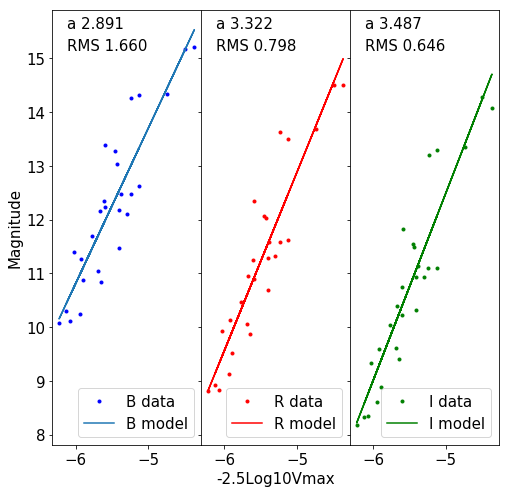
\includegraphics[width=5in]{TF.png}
\caption{Tully-Fisher relations for the Virgo Cluster in B, R, and I bands (left to right). Each panel includes the slope as well as the RMS of the fit}
\end{figure}

\subsection{uncertainties}
Propagating the error in the distance modulus, and taking the apparent magnitude to be well known

$$M = 5\log(d) + -5 = \frac{5 \mathrm{Ln} (d)}{\mathrm{Ln} (10)} - 5$$
$$\sigma_{M} = \frac{5}{\mathrm{Ln} (10)} \frac{\sigma_{d}}{d}$$
$$\sigma_{M} \frac{\mathrm{Ln} (10)}{5} = \frac{\sigma_{d}}{d}$$

For an uncertainty of .25 magnitudes we get a fractional error on distance of 11.5\%, and for an uncertainty of .75 magnitudes we get fractional error on the distance of 34.5\%. The cofactor on sigma m is approximately a half
\section{Exercises with surface brightnesses}
Using the effective radius and scale height we are given for this galaxy, we can write down the surface brightness profiles for the disk and bulge components. 

$$ \Sigma_{B}(r) = \Sigma_{0,b} \exp{-7.67(r/18)^{1/4}},  \Sigma_{D}(r) = \Sigma_{0,d} \exp{-(r/18)} $$

$$ \mu_{disk}(r) =  \mu_{0,d} + 0.06032\, r, \mu_{bulge}(r) =  \mu_{0,b} + 4.04298 \, r^{1/4} $$

Now given $\mu_{bulge}(18) = \mu_{disk}(18) = 22$ we can solve

$$ 22 =  \mu_{0,d} + 0.06032\, (18),  \mu_{0,d} = 20.914$$
$$ 10^{\mu_{0,d}/-2.5} = 10^{20.914/-2.5} =  10^{-8.366}= \Sigma_{0,d} $$
$$ 22 = \mu_{0,b} + 4.04298 \, (18)^{1/4}, \mu_{0,b} = 13.6724  $$
$$ 10^{\mu_{0,b}/-2.5} = 10^{13.6724/-2.5} =  10^{-5.4690}= \Sigma_{0,b}$$

\subsection{Total surface brightness at 18''}
The total surface brightness of the galaxy is the sum of the disk component and the bulge component. Taking magnitudes in the usual way gives us

$$ -2.5\log(\Sigma_{disk}(18) + \Sigma_{bulge}(18)) = -2.5\log(\Sigma_{0,b} \exp(-7.67) + \Sigma_{0,d} \mathrm{e}) = 19.6914 $$

\subsection{Central brightness, disk}
For the central brightnesses of the disk component, we can pick off $\mu_{0,d} = 20.914$ in magnitudes per arcseconds squared. 

To obtain a value in solar luminosities per parsec squared, we have to play around with the distance modulus. We have

$$ m_{B} - M_{B} = 5\log(d(pc)/1pc) - 5 $$

Comparing the absolute magnitude of a source to the sun's absolute magnitude gives us

$$M_{B} - M_{B \odot} = -2.5\log(L / L_{\odot}) $$

We can write L in terms of the luminosity density, I, for a source away a distance d a way $L = I \mathrm{d}A = I d^2 \mathrm{d}\theta^2$. 1'' (1 degree/3600 '') * ($\pi$ rad / 180 degrees) = 4.848e-6 radians. So all together we have

$$ \mu  + 2.5\log(L / L_{\odot}) - M_{B \odot} = 5\log d - 5 $$
$$ \mu  + 2.5\log(Id^2  \times (4.848\times10^{-6})^{2} / L_{\odot}pc^{-2}) - M_{B \odot} = 5\log d - 5 $$
$$ \mu  = -2.5\log Id^2 - 5\log 4.848\times10^{-6} - 2.5\log( I/ L_{\odot}pc^{-2}) + M_{B \odot} + 5\log d - 5 $$
$$ \mu  =  - 5\log 4.848\times10^{-6}  - 2.5\log( 1/ L_{\odot}pc^{-2}) + M_{B \odot}  - 5 $$
$$ \mu  =  21.572 - 2.5\log( I/ L_{\odot}pc^{-2}) + M_{B \odot} $$
$$ \mu  -  21.572 - M_{B \odot} = - 2.5\log( I/ L_{\odot}pc^{-2}) $$
$$ 10^{(\mu  -  21.572 - M_{B \odot})/-2.5} =  I/ L_{\odot}pc^{-2} $$

Now using $\mu_{0,disk} = 20.914$, $M_{B\odot} = 5.48$ gives us 285.23 $L_{\odot} pc^{-2}$. 
\subsection{Central brightness, bulge}

For the central brightness of the bulge we can pick off $\mu_{0,b} = 13.6724$ in magnitudes per arcseconds squared. 

Using this in the expression above to calculate surface brightness in physical units gives us 224491 $L_{\odot} pc^{-2}$
\subsection{Fraction of light below sky background, disk}
For the fractional components we can sum up the area weighted brightness up to the distance at which the surface brightness of the galaxy matches that of the sky background, and normalize by the total luminosity. 

$$ \int^{r}_{0} \Sigma(r') r' \mathrm{d}r' / \int^{\infty}_{0} \Sigma(r') r' \mathrm{d}r' $$
where we have canceled out the angular dependence and central brightnesses.For both the bulge and disk, the surface brightness matches the sky (22 magnitudes/''sq) at a distance of 18 arseconds, so in both cases we integrate out to r=18 in the numerator.

For the exponential component this becomes
$$ \int^{18}_{0} \exp(-r/18)r \mathrm{d}r / \int^{\infty}_{0} \exp(-r/18)r \mathrm{d}r $$
$$ 85.614 / 324 \approx 26.4\%$$

which means 73.4\% of the light from the disk happens at a surface brightness fainter than the sky background.

\subsection{Fraction of light below sky background, bulge}
For the bulge component, the effective radius is supposed to contain half the bulge's light by definition.
$$  \int^{18}_{0} \exp(-7.67(r/18)^{1/4}) r \mathrm{d}r / \int^{\infty}_{0} \exp(-7.67(r/18)^{1/4}) r \mathrm{d}r $$
.272732 / .54537 = .5 as expected. As a result, 50\% of the light from the bulge component happens at a surface brightness fainter than the sky background.

\subsection{Bulge-to-disk ratio}
Binney and Merrifield quote the disk to bulge ratio as $(B/T)^{-1} -1$ where $$(B/T) = \frac{\Sigma_{e,b} r_{e}^{2}}{\Sigma_{e,b} r_{e}^{2} + .28 \Sigma_{0,d}h_{e}^2 }$$

Since the effective radius and scale height are equal in our case, this becomes 

$$\frac{\Sigma_{e,b}}{\Sigma_{e,b}  + .28 \Sigma_{0,d}} = \frac{\exp(-7.67)10^{-5.4690}}{\exp(-7.67)10^{-5.4690}  + .28 \times10^{-8.366}} = .567965$$

where we used $\Sigma_{e}e^{-7.65} = \Sigma_{0}$ for the bulge component. Using this value for $(B/T)$ we get a disk-to-bulge ratio of .761, or a bulge-to-disk ratio of 1.314.

\subsection{Apparent magnitude of disk}
We can use our previous result of the central luminosity in solar luminosity per square parsec, the distance modulus, and absolute magnitude to work out the apparent magnitude. First, we will have to work out the total luminosity of the disk

$$L = 2\pi \int^{\infty}_{0} \Sigma_{0}\exp(-r/h_{r}) r\mathrm{d}r = 2\pi \Sigma_{0}h_{r}^{2} $$

We worked out $\Sigma_{0} =  285.23 L_{\odot} pc^{-2}$ for the disk. In our angular units, we have $h_{r}$ = 18 arcseconds. We can put this into parsecs using the small angle approximation. Since 1AU/1pc = 1'', and 1pc = 206264.8062 AU, if the galaxy is a distance $d$ away in pc the scale height in parsecs is h=18$d$/206264.8062.

$$ m  + 2.5\log(2\pi \Sigma_{0}d^2  \times (18/206264.8062)^{2}) - M_{B \odot} = 5\log d - 5 $$
$$ m  = -2.5\log(\Sigma_{0}) - 2.5\log(2\pi (18/206264.8062)^{2}) + M_{B \odot}   - 5 $$
$$ m  = -2.5\log(\Sigma_{0}) + 18.78 $$

Using the value of the central luminosity we found, we get m = 12.64 (seems a bit bright?)

\subsection{Apparent magnitude of bulge}
Binney and Merrifield work out the total luminosity of a de Vaucoulers profile. Since the effective radius is defined to contain half the light, we can integrate the surface brightness out to $R_{e}$ and multiply by 2.

$$L = 2 \times 2\pi \int^{Re}_{0} \Sigma_{e}(r) r \mathrm{d}r = \frac{8! \exp(7.67)}{(7.67)^{8}}\pi R_{e}^{2} \Sigma_{e} =  \frac{8!\exp(7.67)}{(7.67)^{8}}\pi R_{e}^{2} \Sigma_{0}\exp(-7.67)$$

Now we place our galaxy at a distance d away, and find $R_{e}$ = 18$d$/206264.8062 and stick in our luminosity

$$ m  + 2.5\log[\frac{8!}{(7.67)^{8}}\pi \Sigma_{0} d^2  \times (18/206264.8062)^{2}] - M_{B \odot} = 5\log d - 5 $$
$$ m  = - 2.5\log[\frac{8!}{(7.67)^{8}}\pi \Sigma_{0}  \times (18/206264.8062)^{2}] + M_{B \odot}  - 5 $$

Using $\Sigma_{0} = 224491$ and $M_{B \odot} = 5.48$ gives us an apparent magnitude of 12.34. Fairly close to our result for the disk magnitude. 

\subsection{Apparent magnitude of whole galaxy}

We must add the luminosity of the disk and bulge components together to get an effective luminosity, and follow the same procedure we used in the previous 2 problems. 

$$ m  +  2.5\log[(\frac{8!}{(7.67)^{8}} \Sigma_{0,bulge} + 2 \Sigma_{0, disk}) \pi d^2  \times (18/206264.8062)^{2}] - M_{B \odot} = 5\log d - 5 $$
$$ m  = - 2.5\log[(\frac{8!}{(7.67)^{8}} \Sigma_{0,bulge} + 2 \Sigma_{0, disk}) \pi  \times (18/206264.8062)^{2}] + M_{B \odot}  - 5 $$

plugging in the numbers gives us m = 11.726

\subsection{New bulge-to-disk ratio}
We can revisit our calculation of $\Sigma_{0,bulge}$ from the very beginning of the problem and use a surface magnitude of 21 instead of 22. This gives us

$$ 21 = \mu_{0,b} + 4.04298 \, (18)^{1/4}, \mu_{0,b} = 12.6724  $$
$$ 10^{\mu_{0,b}/-2.5} = 10^{12.6724/-2.5} =  10^{-5.0689}= \Sigma_{0,b}$$

Now we use our new central brightness to calculate 
$$(B/T) = \frac{\Sigma_{e,b}}{\Sigma_{e,b}  + .28 \Sigma_{0,d}} = \frac{\exp(-7.67)10^{-5.0689}}{\exp(-7.67)10^{-5.0689}  + .28 \times10^{-8.366}} = .7676$$

Which yields a disk-to-bulge ratio of .303 or a bulge to disk ratio of 3.3

\subsection{Concentration Parameter}
Lets write up a small program to calculate the total surface brightness and total flux, numerically solve for $R_{25}$, and calculate C30

\begin{lstlisting}[language=Python]
from scipy.optimize import fsolve
import numpy as np

def mag_surf(x):
    '''
    calculate surface magnitude using bulge and disk 
    profiles
    '''
    sig_0_disk = 10**-8.366
    sig_0_bulge = 10**-5.469
    sig_disk = sig_0_disk * np.exp(-x/18.)
    sig_bulge = sig_0_bulge * np.exp(-7.67*(x/18.)**.25)
    return -2.5*np.log10(sig_disk + sig_bulge)

def mag():
    '''
    return the surface brightness magnitude 
    we're looking for
    '''
    return 25

def findIntersection(fun1,fun2,x0):
    '''
    numerically find the intersection of 2 functions
    '''
    return fsolve(lambda x : fun1(x) - fun2(),x0)

#calculate R25, use the effective radius as an initial guess
R25 = findIntersection(mag_surf, mag, 18)

#calculate C30


import scipy.integrate as integrate
def surf_bright(x):
    '''
    calculate surface brightness
    '''
    sig_0_disk = 10**-8.366
    sig_0_bulge = 10**-5.469
    return sig_0_disk * np.exp(-(x)/18.) + sig_0_bulge * np.exp(-7.67*((x)/18.)**.25)

#find the flux inside .3R25 by integrating over the surface brightness
#and dividing by angular area
numerator = integrate.quad(lambda x: surf_bright(x) ,0,.3*R25) /(.3*R25)**2
#find flux inside R25
denominator= integrate.quad(lambda x: surf_bright(x),0,R25) /(R25)**2

#calculate C30
print numerator[0]/denominator[0]
\end{lstlisting}
gives a C30 of 10.379

We can run the program over again, but swapping out \texttt{sig\_0\_bulge} =  10**-5.0689, the new central brightness we found when we calculated the second bulge to disk ratio, and we get a C30 of 10.697. The second galaxy is bulge-ier, which is consistent with what we found previously. However, the ratio differed by almost a factor of 3 in the previous problems. so I probably messed up somewhere. Also, the bulge to disk ratios were of order unity, and the C30s here are of order 10. So I'm pretty sure I messed up somewhere, though I can't find my mistake :(

\end{document}